\ifdefined \buildingFullOPALManual \else


%\ifx \@buildingFullOPALManual \@empty
%\else

%\documentclass[12pt,a4paper]{report}
\documentclass[a4paper]{book}

%% does not work in Latex2Html mode
%\usepackage{hyperref}

\usepackage[T1]{fontenc}
\usepackage{url}
\usepackage{html}
\usepackage{epic}
\usepackage{eepic}
\usepackage{makeidx}
\usepackage{array}
\usepackage{times}
\usepackage{amsmath}
\usepackage{amsxtra}
\usepackage{bm}
\usepackage[thin,thinp,thinc]{esdiff}
\usepackage{graphicx}
\usepackage{dingbat}
\usepackage{color}
\usepackage{subfig}
\usepackage{boxedminipage}
\usepackage{alltt}
\usepackage{nicefrac}
\usepackage{calc}
%\usepackage{pdfdraftcopy}             % Draft
\usepackage{tikz}
\usetikzlibrary{
  er,3d,calc,fadings,trees,positioning,arrows,chains,decorations.pathreplacing,
  decorations.pathmorphing,shapes,shapes.symbols,shapes.arrows,matrix,through,decorations.text
}

\tikzset{
  >=stealth',
  punktchain/.style={rectangle,rounded corners, draw=black, very thick,text width=10em,
                     minimum height=3em, text centered, on chain},
  line/.style={draw, thick, <-},
  element/.style={tape,top color=white,bottom color=blue!50!black!60!,minimum width=8em,
                  draw=blue!40!black!90, very thick,text width=10em, minimum height=3.5em,
                  text centered, on chain},
  every join/.style={->, thick,shorten >=1pt},
  tuborg/.style={decorate},
  tubnode/.style={midway, right=2pt}
}

\tikzstyle{material}=[draw, fill=blue!20, text width=16.0em, text centered, minimum height=1.5em]
\tikzstyle{diagramstep} = [material, text width=20em, minimum width=10em, minimum height=3em, rounded corners]
\tikzstyle{line} = [draw, thick, color=black!50, -latex']

\usepackage{booktabs}
\usepackage{xspace}
\usepackage{xstring}

\usepackage{fancyvrb}
\usepackage{rotating}
\usepackage{float}

\usepackage{tabularx}
\usepackage{longtable}
\setcounter{LTchunksize}{3}

\usepackage[section]{placeins}
\usepackage{MnSymbol}
\usepackage{microtype}
\usepackage{setspace}
\usepackage{dcolumn}

\usepackage[vmargin={3.0cm,3.0cm},
            hmargin={2.0cm,3.0cm}]{geometry}

\usepackage{upgreek}
\usepackage[binary-units=true]{siunitx}
\sisetup{exponent-product = \cdot,math-ohm=\Upomega,text-ohm=\ensuremath{\Upomega}}
\DeclareSIUnit{\clight}{c}
\DeclareSIUnit\gauss{Ga}

\usepackage{engord}
\usepackage{wasysym}
\DeclareSIUnit[number-unit-product = \,]{\permill}{\permil}

\usepackage{hyperref}
\hypersetup{
    pdftitle          = The OPAL Framework,
    pdfauthor         = {Andreas Adelmann, Achim Gsell, Valeria Rizzoglio, Christof Metzger-Kraus,
                         Yves Ineichen, Xiaoying Pang, Steve Russell, Chuan Wang, Jianjun Yang,
                         Suzanne Sheehy, Chris Rogers, Daniel Winklehner},
    pdfsubject        = User's Reference Manual,
    pdffitwindow      = true,               % page fit to window when opened
    pdfnewwindow      = true,               % links in new window
    colorlinks        = true,               % false: boxed links; true: colored links
    linkcolor         = black!80!green,     % color of internal links
    citecolor         = black!20!red,       % color of links to bibliography
    urlcolor          = blue,               % color of external links
    breaklinks        = true,
    bookmarksnumbered = true,
    plainpages        = false
}

\usepackage{ifthen}

\newif \iflinuxwindows
\linuxwindowstrue   % set this to true when building the manual on Linux or Windows
\iflinuxwindows
\usepackage{epstopdf}
\fi

\usepackage[backend=biber,
            style=phys,
            biblabel=brackets,
            maxnames=3,
            doi=true,
            isbn=true,
            url=true]{biblatex}
%---- macros ----

\renewcommand{\topfraction}{1.0}
\renewcommand{\bottomfraction}{1.0}
\renewcommand{\textfraction}{0.0}
\renewcommand{\arraystretch}{2.0}
\newenvironment{tex2html_nowrap}{}{}


\newcommand{\Newline}{\hfil \\}


\newsavebox{\ExampleBox}
\newenvironment{example}
 {\VerbatimEnvironment
  \begin{flushleft}
  \begin{lrbox}{\ExampleBox}
    \begin{minipage}{\linewidth}
  \begin{Verbatim}[frame=lines,xleftmargin=0cm,fontsize=\footnotesize,samepage=true]}
 {\end{Verbatim}
  \end{minipage}
  \end{lrbox}
  \mbox{\usebox{\ExampleBox}}
  \end{flushleft}
 }

\newenvironment{longexample}
{\Verbatim[frame=lines,xleftmargin=0mm,fontsize=\footnotesize]}
{\endVerbatim}

%\examplefromfile{filename} reads in a text file and displays it in the document.
\newcommand{\examplefromfile}[1]{
\VerbatimInput[frame=lines,xleftmargin=0mm,fontsize=\footnotesize,label=\texttt{#1}]{#1}}

%for upright d of differentials
\makeatletter
\newcount\my@repeat@count

\newcommand{\myrepeat}[2]{%
  \begingroup
  \my@repeat@count=\z@
  \@whilenum\my@repeat@count<#1\do{#2\advance\my@repeat@count\@ne}%
  \endgroup
}

\newcommand{\differential}[1]{\ifstrempty{#1}{\ES@dop\ES@difint}{\ES@dop^{#1}\ES@difint}}
\newcommand{\pdifferential}[1]{\ifstrempty{#1}{{\partial\,}}{{\partial^{#1}\,}}}

\makeatother

\newcommand{\der}[3][]{\frac{\differential{#1}#2}{\differential{}\ifstrempty{#1}{#3}{#3^#1}}}
\newcommand{\parder}[3][]{\frac{\pdifferential{#1}#2}{\pdifferential{}\ifstrempty{#1}{#3}{#3^#1}}}
\newcommand{\niceder}[3][]{\nicefrac{\differential{#1}#2}{\differential{}\ifstrempty{#1}{#3}{#3^#1}}}
\newcommand{\uglyder}[3][]{{\differential{#1}#2}/{\differential{}\ifstrempty{#1}{#3}{#3^#1}}}
\newcommand{\uglyparder}[3][]{{\pdifferential{#1}#2}/{\pdifferential{}\ifstrempty{#1}{#3}{#3^#1}}}
\newcommand{\dd}[1][]{\; \differential{#1}}
\newcommand{\primed}{^{\prime}}
\newcommand{\dprimed}{^{\prime\prime}}
\newcommand{\nprimed}[1]{^{\myrepeat{#1}{\prime}}}

%Editing Macros
\newcommand{\TODO}[1]{{\color{red}\ifthenelse{\boolean{ShowDebug}}{[TODO: #1]}{}}}



%text in gray box
\newsavebox{\fmbox}
\definecolor{lightgray}{gray}{0.95}
\newenvironment{fmpage}
   {\vspace{-1.0cm}\begin{lrbox}{\fmbox}\begin{minipage}[t]{13.5cm}\vspace{0.1cm}}
   {\vspace{-0.4cm}\end{minipage}\end{lrbox}\begin{center}\fcolorbox{black}{lightgray}{\usebox{\fmbox}}\end{center}}


% Definition new signes
\newcommand{\R}{{\mathbb R}} % real numbers
\newcommand{\Q}{{\mathbb Q}} % rational numbers
\newcommand{\Z}{{\mathbb Z}} % integer numbers
\newcommand{\N}{{\mathbb N}} % natural numbers

\newcommand{\mad}{\textsc{mad}\xspace}
\newcommand{\madnine}{\textsc{mad9}\xspace}
\newcommand{\madninep}{\textsc{mad9p}\xspace}
\newcommand{\madeight}{\textsc{mad8}\xspace}
\newcommand{\classic}{\textsc{classic}\xspace}

\makeatletter
\newcommand{\opal@impl}{\textsc{Opal}}
\newcommand{\opalt@impl}{\textsc{Opal-t}}
\newcommand{\opalcycl@impl}{\textsc{Opal-cycl}}
\newcommand{\opalmap@impl}{\textsc{Opal-map}}
\newcommand{\opalenv@impl}{\textsc{Opal-e}}

\newcommand{\opal}{\opal@impl\xspace}
\newcommand{\opalt}{\opalt@impl\xspace}
\newcommand{\opalcycl}{\opalcycl@impl\xspace}
\newcommand{\opalmap}{\opalmap@impl\xspace}
\newcommand{\opalenv}{\opalenv@impl\xspace}

\newcommand{\noopalt}{\leftthumbsdown \opalt@impl\xspace}
\newcommand{\noopalcycl}{\leftthumbsdown \opalcycl@impl\xspace}
\newcommand{\noopalmap}{\leftthumbsdown \opalmap@impl\xspace}
\newcommand{\noopalenv}{\leftthumbsdown \opalenv@impl\xspace}
\makeatother

\newcommand{\impactt}{\textsc{Impact-t}\xspace}
\newcommand{\partroot}{\textsc{H5root}}


\newcommand{\latermore}{More details will be given in Version 1.6.0}


\newcommand{\lieop}[1]{{:}{#1}{:}}

\newcommand{\rms}[1]{\overset{\sim}{#1}}

\newcommand{\sprod}{\cdot}
\newcommand{\vprod}{\times}
\newcommand{\matr}[1]{\mathcal{#1}}
\renewcommand{\vec}[1]{{\bm{#1}}}
\newcommand{\transpose}[1]{#1^\intercal}
\renewcommand{\epsilon}{\varepsilon}

\newcommand{\keyword}[2][]{\ifstrempty{#1}{\texttt{\expandafter\MakeUppercase\expandafter{#2}}}{\hyperref[#1]{\texttt{\expandafter\MakeUppercase\expandafter{#2}}}}}
\newcommand{\tabline}[3][]{\keyword[#1]{#2}& #3 \\}
\newcommand{\tabheadcell}[1]{{\bfseries #1}}

\newcommand*\kdescriptionlabel[1]{\hspace\labelsep
                                \normalfont\keyword{#1}\index{#1}}
\makeatletter
\newenvironment{kdescription}
               {\list{}{\labelwidth\z@ \itemindent-\leftmargin
                        \let\makelabel\kdescriptionlabel}}
               {\endlist}
\makeatother

\ExplSyntaxOn
\NewDocumentCommand{\tabhead}{ m }
 {
  \seq_set_split:Nnn \l_tmpa_seq { & } { #1 }
  \bfseries \seq_use:Nn \l_tmpa_seq { & \bfseries } \\
 }

\NewDocumentCommand \multrefImpl { O{ } m m m } {
  \ifnumgreater{\clist_count:n {#4}}{1}{
    \seq_set_from_clist:Nn \l_tmpa_seq { #4 }

    \seq_set_map:NNn \l_tmpb_seq \l_tmpa_seq { \exp_not:n { \ref{#3:##1} } }
    \ifstrempty{#1}{#2s}{#1}~\seq_use:Nnnn \l_tmpb_seq {\ and\ } {,\ } {,\ and\ }
  }{
    #2~\ref{#3:#4}
  }
}

\NewDocumentCommand \multeqnrefImpl { m } {
  \ifnumgreater{\clist_count:n {#1}}{1}{
    \seq_set_from_clist:Nn \l_tmpa_seq { #1 }

    \seq_set_map:NNn \l_tmpb_seq \l_tmpa_seq { \exp_not:n { \eqref{eq:##1} } }
    Equations~\seq_use:Nnnn \l_tmpb_seq {\ and\ } {,\ } {,\ and\ }
  }{
    Equation~\eqref{eq:#1}
  }
}
\ExplSyntaxOff


%Abbreviations for Equations, Figures, and Tables
%\newcommand{\Equation}[1]{Equation~\eqref{#1}}

\newcommand{\bibref}[2]{#1 \cite{bib:#2}}
\newcommand{\figref}[1]{\multrefImpl{Figure}{fig}{#1}}
\newcommand{\chpref}[1]{\multrefImpl{Chapter}{chp}{#1}}
\newcommand{\appref}[1]{\multrefImpl[Appendices]{Appendix}{chp}{#1}}
\newcommand{\secref}[1]{\multrefImpl{Section}{sec}{#1}}
\newcommand{\ssecref}[1]{\multrefImpl{Section}{ssec}{#1}}
\newcommand{\tabref}[1]{\multrefImpl{Table}{tab}{#1}}
\newcommand{\eqnref}[1]{\multeqnrefImpl{#1}}

\newcommand{\seefig}[1]{(see~\figref{#1})}
\newcommand{\seechp}[1]{(see~\chpref{#1})}
\newcommand{\seesec}[1]{(see~\secref{#1})}
\newcommand{\seessec}[1]{(see~\ssecref{#1})}
\newcommand{\seetab}[1]{(see~\tabref{#1})}
\newcommand{\seeeqn}[1]{(see~\eqnref{#1})}

\newcommand{\filename}[1]{\emph{#1}}


% Define distances for bordering
\newcommand{\blockdist}{1.3}
\newcommand{\edgedist}{1.5}
\newcommand{\diagramstep}[2]{node (p#1) [diagramstep] {#2}}


% place chapter title page on odd pages
\let\stdchapter\chapter
\makeatletter
\renewcommand*{\chapter}{\if@openright\cleardoublepage\else\clearpage\fi\stdchapter}

\makeatother

\IfFileExists{./version.tex}{%
  \newcommand{\opalversion}[1]{Version \ifstrempty{#1}{1.9.0}{#1}\xspace}
%
}%
{%
  \newcommand{\opalversion}[1]{\ifstrempty{#1}{current Version}{Version #1}\xspace}%
}
\newboolean{ShowMap}
\setboolean{ShowMap}{false}

\newboolean{ShowEnv}
\setboolean{ShowEnv}{false}

\newboolean{ShowDebug}
\setboolean{ShowDebug}{false}

%----Control Structures
\newboolean{FullOPALManual}
\setboolean{FullOPALManual}{false}


\makeindex


\bibliography{bibliography}
\begin{document}

\fi

\chapter{Auto-phasing Algorithm}
\label{chp:autophasing}
%\index{Autophase Algorithm}

\section{Standing Wave Cavity}
\index{Autophase Algorithm!Standing Wave Cavity}
In \opalt the elements are implemented as external fields that are read in from a file. The fields are described by a 1D, 2D or 3D sampling (equidistant or non-equidistant). To get the actual field at any position a linear interpolation multiplied by $\cos(\omega t + \varphi)$, where $\omega$ is the frequency and $\varphi$ is the lag. The energy gain of a particle then is
\begin{equation}
\Delta E(\varphi,r) = q\,V_{0}\,\int_{z_\text{begin}}^{z_\text{end}} \cos(\omega t(z,\varphi) + \varphi) E_z(z, r) dz.
\end{equation}
To maximize the energy gain we have to take the derivative with respect to the lag, $\varphi$ and set the result to zero:
\begin{multline}
\differential{\Delta E(\varphi,r)}{\varphi} = -\int_{z_\text{begin}}^{z_\text{end}} (1 + \omega \diffp{t(z,\varphi)}{\varphi}) \sin(\omega t(z,\varphi) + \varphi) E_z(z,r)\\
= -\cos(\varphi) \int_{z_\text{begin}}^{z_\text{end}} (1 + \omega \diffp{t(z,\varphi)}{\varphi}) \sin(\omega t(z,\varphi)) E_z(z,r) dz \\
-\sin(\varphi) \int_{z_\text{begin}}^{z_\text{end}} (1 + \omega \diffp{t(z,\varphi)}{\varphi}) \cos(\omega t(z,\varphi)) E_z(z,r) dz \stackrel{!}{=} 0.
\end{multline}
Thus to get the maximum energy the lag has to fulfill
\begin{equation} \label{eq:rulelag}
  \tan(\varphi) = -\frac{\Gamma_1}{\Gamma_2},
\end{equation}
where
\begin{equation}
  \label{eq:Gamma1}
  \Gamma_1 = \sum_{i=1}^{N-1} (1 + \omega \diffp{t}{\varphi}) \int_{z_{i-1}}^{z_{i}} \sin\left(\omega (t_{i-1} + \Delta t_{i}\frac{z-z_{i-1}}{\Delta z_{i}})\right)\left(E_{z,i-1} + \Delta E_{z,i} \frac{z-z_{i-1}}{\Delta z_{i}}\right) dz
\end{equation}
and
\begin{equation}
  \label{eq:Gamma2}
  \Gamma_2 = \sum_{i=1}^{N-1} (1 + \omega \diffp{t}{\varphi}) \int_{z_{i-1}}^{z_{i}} \cos\left(\omega (t_{i-1} + \Delta t_{i}\frac{z-z_{i-1}}{\Delta z_{i}})\right)\left(E_{z,i-1} + \Delta E_{z,i} \frac{z-z_{i-1}}{\Delta z_{i}}\right) dz.
\end{equation}
Between two sampling points we assume a linear correlation between the electric field and position respectively between time and position. The products in the  integrals between two sampling points can be expanded and solved analytically. We then find
\begin{equation*}
\Gamma_1 = \sum_{i=1}^{N-1} (1 + \omega \diff{t}{\varphi}) \Delta z_{i}(E_{z,i-1} (\Gamma_{11,i} - \Gamma_{12,i}) + E_{z,i}\, \Gamma_{12,i})
\end{equation*}
and
\begin{equation*}
\Gamma_1 = \sum_{i=1}^{N-1} (1 + \omega \diffp{t}{\varphi}) \Delta z_{i}(E_{z,i-1} (\Gamma_{21,i} - \Gamma_{22,i}) + E_{z,i}\, \Gamma_{22,i})
\end{equation*}
where
\begin{align*}
  \Gamma_{11,i} &= \int_0^1 \sin(\omega(t_{i-1} + \tau \Delta t_{i})) d\tau = - \frac{\cos(\omega t_{i}) - \cos(\omega t_{i-1})}{\omega \Delta t_{i}}\\
  \Gamma_{12,i} &= \int_0^1 \sin(\omega(t_{i-1} + \tau \Delta t_{i})) \tau d\tau = \frac{-\omega \Delta t_{i} \cos(\omega t_{i}) + \sin(\omega t_{i}) - \sin(\omega t_{i-1})}{\omega^2 (\Delta t_{i})^2}\\
  \Gamma_{21,i} &= \int_0^1 \cos(\omega(t_{i-1} + \tau \Delta t_{i})) d\tau = \frac{\sin(\omega t_{i}) - \sin(\omega t_{i-1})}{\omega \Delta t_{i}}\\
  \Gamma_{22,i} &= \int_0^1 \cos(\omega(t_{i-1} + \tau \Delta t_{i})) \tau d\tau = \frac{\omega \Delta t_{i} \sin(\omega t_{i}) + \cos(\omega t_{i}) - \cos(\omega t_{i-1})}{\omega^2 (\Delta t_{i})^2}
\end{align*}

It remains to find the progress of time with respect to the position. In \opal this is done iteratively starting with
\begin{verbatim}
K[i] = K[i-1] + (z[i] - z[0]) * q * V;
b[i] = sqrt(1. - 1. / ((K[i] - K[i-1]) / (2.*m*c^2) + 1)^2);
t[i] = t[0] + (z[i] - z[0]) / (c * b[i])
\end{verbatim}
By doing so we assume that the kinetic energy, K, increases linearly and proportional to the maximal voltage. With this model for the progress of time we can calculate $\varphi$ according to \eqnref{rulelag}. Next a better model for the kinetic Energy can be calculated using
\begin{alltt}
K[i] = K[i-1] + q \(\Delta\)z[i](cos(\(\varphi\))(Ez[i-1](\(\Gamma\sb{21}\)[i] - \(\Gamma\sb{22}\)[i]) + Ez[i]\(\Gamma\sb{22}\)[i])
                      \(\,\,\)- sin(\(\varphi\))(Ez[i-1](\(\Gamma\sb{11}\)[i] - \(\Gamma\sb{12}\)[i]) + Ez[i]\(\Gamma\sb{12}\)[i])).
\end{alltt}
With the updated kinetic energy the time model and finally a new $\varphi$, that comes closer to the actual maximal kinetic energy, can be obtained. One can iterate a few times through this cycle until the value of $\varphi$ has converged.

\section{Traveling Wave Structure}
\index{Autophase Algorithm!Traveling Wave Structure}
\begin{figure}
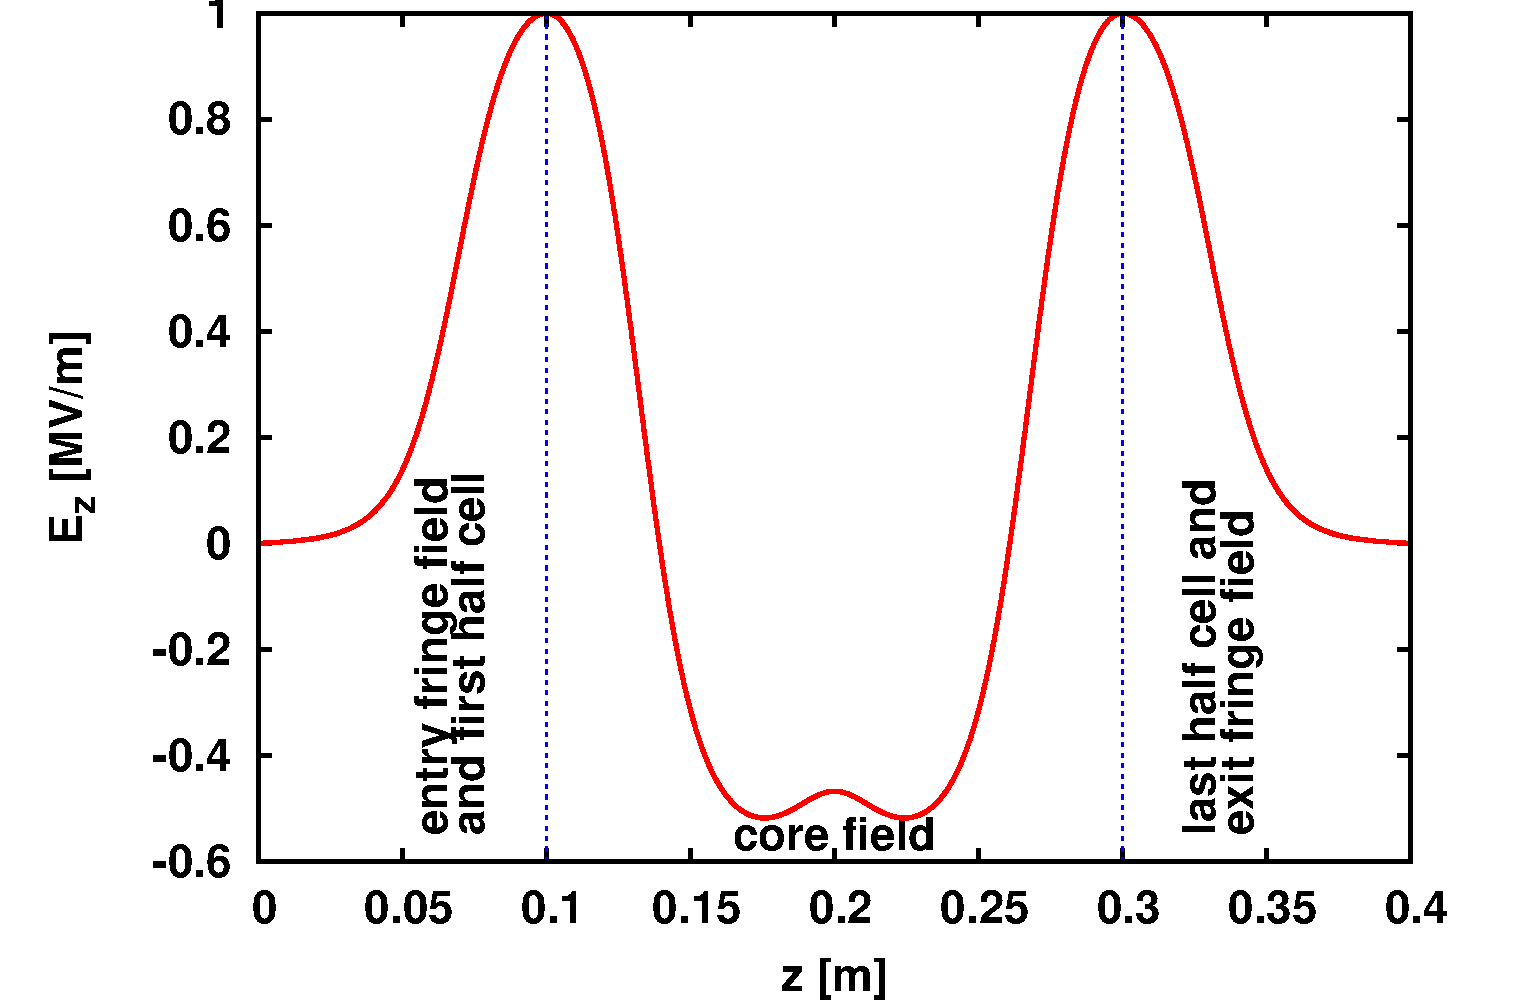
\includegraphics[angle=0,width=0.9\linewidth]{figures/field_crop}
\caption{Field map 'FINLB02-RAC.T7' of type 1DDynamic}
\label{fig:tws}
\end{figure}
Auto phasing in a traveling wave structure is just slightly more complicated. The field of this element is composed of a standing wave entry and exit fringe field and two standing waves in between, see \figref{tws}.
\begin{multline}
\Delta E(\varphi,r) = q\, V_{0}\,\int_{z_\text{begin}}^{z_\text{beginCore}} \cos(\omega t(z,\varphi) + \varphi) E_z(z, r) dz \\
+ q\, V_\text{core}\,\int_{z_\text{beginCore}}^{z_\text{endCore}} \cos(\omega t(z,\varphi) + \varphi_\text{c1} + \varphi) E_z(z, r) dz \\
+ q\, V_\text{core}\,\int_{z_\text{beginCore}}^{z_\text{endCore}} \cos(\omega t(z,\varphi) + \varphi_\text{c2} + \varphi) E_z(z + s, r) dz \\
+ q\, V_{0}\,\int_{z_\text{endCore}}^{z_\text{end}} \cos(\omega t(z,\varphi) + \varphi_\text{ef} + \varphi) E_z(z, r) dz,
\end{multline}
where $s$ is the cell length. Instead of one sum as in \eqnref{Gamma1,Gamma2} there are four sums with different numbers of summands.
\subsection*{Example}
\begin{fmpage}
\begin{verbatim}
FINLB02_RAC: TravelingWave, L=2.80, VOLT=14.750*30/31, NUMCELLS=40,
             FMAPFN="FINLB02-RAC.T7", ELEMEDGE=2.67066, MODE=1/3,
             FREQ=1498.956, LAG=FINLB02_RAC_lag;
\end{verbatim}
\end{fmpage}
For this example we find
\begin{align*}
  V_\text{core} &= \frac{V_{0}}{\sin(2.0/3.0 \pi)} = \frac{2 V_{0}}{\sqrt{3.0}}\\
  \varphi_\text{c1} &= \frac{\pi}{6}\\
  \varphi_\text{c2} &= \frac{\pi}{2}\\
  \varphi_\text{ef} &= - 2\pi \cdot(\text{\keyword{NUMCELLS}} - 1) \cdot \text{\keyword{MODE}} = 26\pi
\end{align*}
\subsection{Alternative Approach for Traveling Wave Structures}
If $\beta$ doesn't change much along the traveling wave structure (ultra relativistic case) then $t(z,\varphi)$ can be approximated by $t(z,\varphi)=\frac{\omega}{\beta c}z + t_{0}$. For the example from above the energy gain is approximately
\begin{multline*}
\Delta E(\varphi,r) = q\;V_0 \int_{0}^{1.5\cdot s} \cos\left(\omega \left(\frac{z}{\beta c} + t_{0}\right) + \varphi\right) E_z(z,r)\, dz\\
+ \frac{2 q\;V_{0}}{\sqrt{3}} \int_{1.5\cdot s}^{40.5\cdot s}\cos\left(\omega \left(\frac{z}{\beta c} + t_{0}\right) + \frac{\pi}{6} + \varphi \right) E_z(z\;\;\quad,r) dz\\
+ \frac{2 q\;V_{0}}{\sqrt{3}} \int_{1.5\cdot s}^{40.5\cdot s}\cos\left(\omega \left(\frac{z}{\beta c} + t_{0}\right) + \frac{\pi}{2} + \varphi \right) E_z(z+s,r) dz \\
  + q\;V_{0} \int_{40.5\cdot s}^{42\cdot s} \cos\left(\omega \left(\frac{z}{\beta c} + t_{0}\right) + \varphi\right) E_z(z,r)\, dz.
\end{multline*}
Here $\beta c = 2.9886774\cdot10^8\;\text{m s}^{-2}$, $\omega = 2\pi\cdot 1.4989534\cdot10^9$~Hz and, the cell length, $s = 0.06\bar{6}$~m. To maximize this energy we have to take the derivative with respect to $\varphi$ and set the result to $0$. We split the field up into the core field, $E_z^{(1)}$ and the fringe fields (entry fringe field plus first half cell concatenated with the exit fringe field plus last half cell), $E_z^{(2)}$. The core fringe field is periodic with a period of $3\,s$. We thus find
\begin{multline*}
0 \stackrel{!}{=} \int_{0}^{1.5\cdot s} \sin\left(\omega \left(\frac{z}{\beta c} + t_{0}\right) + \varphi\right) E_z^{(2)}(z,r)\, dz \\
                + \frac{2}{\sqrt{3}} \int_{0}^{39\cdot s}\sin\left(\omega \left(\frac{z + 1.5\,s}{\beta c} + t_{0}\right) + \frac{\pi}{6} + \varphi \right) E_z^{(1)}(z \text{ mod}(3\,s)\;\;\qquad,r)\,dz \\
                + \frac{2}{\sqrt{3}} \int_{0}^{39\cdot s}\sin\left(\omega \left(\frac{z + 1.5\,s}{\beta c} + t_{0}\right) + \frac{\pi}{2} + \varphi \right) E_z^{(1)}((z + s) \text{ mod} (3\,s),r)\, dz \\
                + \int_{1.5\cdot s}^{3\cdot s} \sin\left(\omega\left(\frac{z + 39\,s}{\beta c} + t_{0}\right) + \varphi\right) E_z^{(2)}(z,r)\, dz
\end{multline*}
This equation is much simplified if we take into account that $\omega / \beta c \approx 10\pi$. We then get
\begin{multline*}
0 \stackrel{!}{=} \int_{0}^{3\cdot s} \sin\left(\omega \left(\frac{z}{\beta c} + t_{0}\right) + \varphi\right) E_z^{(2)}(z)\, dz \\
                + \frac{26}{\sqrt{3}} \int_{0}^{3\cdot s}\left(\sin\left(\omega \left(\frac{z}{\beta c} + t_{0}\right) + \frac{7\pi}{6} + \varphi \right)
                                                        + \sin\left(\omega \left(\frac{z}{\beta c} + t_{0}\right) + \frac{5\pi}{6} + \varphi \right)\right) E_z^{(1)}(z)\, dz \\
       = \int_{0}^{3\cdot s}\sin\left(\omega \left(\frac{z}{\beta c} + t_{0}\right) + \varphi\right) \left(E_z^{(2)} - 26\cdot E_z^{(1)}\right)(z)\,dz
\end{multline*}
where we used
\begin{multline*}
\int_{0}^{3\cdot s} \sin\left(\omega \left(\frac{z}{\beta c} + t_{0}\right) + \frac{3\pi}{2} + \varphi\right) E_z^{(1)}((z + s) \text{ mod}(3\,s),r) dz \\
\stackrel{z' = z + s}{\longrightarrow} \int_{s}^{4\cdot s} \sin\left(\omega \left(\frac{z'-s}{\beta c} + t_{0} \right) + \frac{3\pi}{2} + \varphi\right)E_z^{(1)}(z' \text{ mod}(3\,s),r)dz' \\
= \int_{0}^{3\cdot s} \sin\left(\omega \left(\frac{z}{\beta c} + t_{0}\right) + \frac{5\pi}{6} + \varphi\right) E_z^{(1)}(z,r)\,dz.
\end{multline*}
In the last equal sign we used the fact that both functions, $\sin(\frac{\omega}{\beta c}z)$ and $E_z^{(1)}$ have a periodicity of $3\cdot s$ to shift the boundaries of the integral.

Using the convolution theorem we find
\begin{equation*}
0 \stackrel{!}{=} \int_{0}^{3\cdot s} g(\xi - z) (G - 26 \cdot H)(z) \, dz =
\mathcal{F}^{-1}\left(\mathcal{F}(g)\cdot(\mathcal{F}(G) - 26 \cdot \mathcal{F}(H))\right)
\end{equation*}
where
\begin{align*}
  g(z) & =
  \begin{cases}
    -\sin\left(\omega \left(\frac{z}{\beta c} + t_{0}\right)\right)\qquad & 0 \le z \le 3\cdot s\\
    0                                     & \text{otherwise}
  \end{cases}\\
  G(z) & =
  \begin{cases}
    E_z^{(2)}(z) \qquad & 0 \le z \le 3\cdot s\\
    0                   & \text{otherwise}
  \end{cases}\\
  H(z) & =
  \begin{cases}
    E_z^{(1)}(z) \qquad & 0 \le z \le 3\cdot s\\
    0                   & \text{otherwise}
  \end{cases}
  \intertext{and}
  -\frac{\omega}{\beta c} \xi &= \varphi.
\end{align*}
Here we also used some trigonometric identities:
\begin{multline*}
  \sin\left(\omega \left(\frac{z}{\beta c} + t_{0}\right) + \pi + \frac{\pi}{6} + \varphi \right) +
  \sin\left(\omega \left(\frac{z}{\beta c} + t_{0}\right) + \pi - \frac{\pi}{6} + \varphi \right) \\
  = -\left(\sin\left(\omega \left(\frac{z}{\beta c} + t_{0}\right) + \frac{\pi}{6} + \varphi\right) +
    \sin\left(\omega \left(\frac{z}{\beta c} + t_{0}\right) - \frac{\pi}{6} + \varphi\right)\right) \\
  = -2\cdot \cos\left(\frac{\pi}{6}\right) \sin\left(\omega \left(\frac{z}{\beta c} + t_{0}\right) + \varphi\right) \\
  = -\sqrt{3} \sin\left(\omega \left(\frac{z}{\beta c} + t_{0}\right) + \varphi\right)
\end{multline*}

%----------- Footer control ------------------
\ifthenelse{\boolean{FullOPALManual}}
{
  %do nothing
}
% else (for individual document creation)
{
\appendix
\printbibliography
\end{document}
}
%---------------------------------------------